%!TEX program = xelatex
% 完整编译: xelatex -> bibtex -> xelatex -> xelatex
\documentclass[lang=cn,11pt,a4paper,cite=authoryear]{elegantpaper}

\title{絮凝体DLA、RLA模型的分形维度影响因素探究}
\author{闵乐钧 519030910326\\ 上海交通大学致远学院计算机方向}

\date{\zhtoday}


% 本文档命令
\usepackage{array}
\newcommand{\ccr}[1]{\makecell{{\color{#1}\rule{1cm}{1cm}}}}

\begin{document}

\maketitle

\begin{center}
    同组成员:孙晨曦,季利恒,严含冲
\end{center}

\begin{abstract}
本文针对三维絮凝体的DLA模型,使用matlab进行模拟凝聚并探究凝聚时间、初始粒子体积密度、布朗运动步长对絮凝体分形维数的影响。在RLA模型中,探究碰撞凝聚概率对分形维数的影响。模拟结果显示这些因素均不存在对分形维数显著的影响,说明一定终止条件下,絮凝体的分形维数是一个固定特征值。
\keywords{DLA,RLA,matlab,分形维数}
\end{abstract}

\section{实验背景和原理介绍}

\subsection{DLA和RLA}
絮体是用絮凝法处理水时水中的胶体和颗粒与絮凝剂相互作用的一种生成物。由于水体运动环境的不可预测性,我们很难通过常规意义下的力学来进行模拟。絮凝过程因而是一个随机的非线性过程,而如何预测这种过程以及测量、描述絮凝体的结构成为一个难题。在20世纪80年代后,新发展而来的分形数学理论得到了较完善的阐发,能够引入到絮凝体形态学研究领域,成为描述絮凝体结构的重要理论推动;另一方面,计算机的迅速发展使得大量的模拟运算成为可能。

DLA(Diffusion-limited aggregation)模型即为计算机模拟絮凝体凝聚的一个经典模型。在有限空间中,预先随机放置粒子,让它们做布朗运动。两个粒子碰撞之后会粘连在一起,随着时间推进而形成具有分形特性的絮凝体。\footnote{Diffusion-limited aggregation, wikipedia, https://en.wikipedia.org/wiki/Diffusion-limited\_aggregation}

DLA模拟的步骤如下:
\begin{enumerate}
    \item 设置立方体空间线度$L$,粒子半径$r$,粒子布朗运动步长$l$(与温度正相关),总粒子数$n$。初始时,在立方体中随机无重叠地放置粒子。
    \item 每个单位时间,让粒子作随机布朗运动。当两个粒子在这个单位时间之后有重叠(说明发生碰撞),则让这两个粒子凝聚在一起,不再做相对运动,并视为一个团簇。
    \item 一定时间之后,模拟终止并计算各种参数。
\end{enumerate}

RLA(Reaction-limited aggregation)模型在DLA模型的基础上,考虑了每次碰撞粘连的概率。即在步骤2中,两个粒子发生碰撞将有概率凝聚。

\subsection{分形维数计算方法}
分形通常被定义为“一个粗糙或零碎的几何形状,可以分成数个部分,且每一部分都(至少近似地)是整体缩小后的形状”,即具有自相似的性质。\footnote{分形,维基百科,https://zh.wikipedia.org/zh-hans/分形}絮凝体的分形形态意味着其结构的紧凑度和可沉降性,因此具有重要的意义。本实验中采用回转半径法计算分形维数。

本模拟实验中,设定每个粒子的质量为1,则全部例子的总质量即为粒子数$n$。在三维多粒子系统中,可通过所有粒子的位置来计算得到回转张量(gyration tensor),
\begin{equation}
    G = \frac{1}{n}\sum\limits_{i = 1}^n
    \left(
        \begin{matrix}
            x_ix_i & x_iy_i & x_iz_i\\
            y_ix_i & y_iy_i & y_iz_i\\
            z_ix_i & z_iy_i & z_iz_i
        \end{matrix}
    \right)
\end{equation}
其中\((x_i, y_i, z_i)\)是第$i$个粒子关于粒子质心的位置矢量。

求出回转张量的三个特征根$\lambda_i, i = 1, 2, 3$,可计算得到系统的回转半径(radius of gyration)
\begin{equation}
    R_g = \sqrt{\lambda_1^2 + \lambda_2^2 + \lambda_3^2}
\end{equation}

由豪斯多夫维数(Hausdorff dimension)的计算方法知,粒子数和其回转半径满足如下关系
\begin{equation}
    n = kR_g^{d_f}
\end{equation}
其中$d_f$即为所求的多孔体系分形维数(Fractal dimension)。在实验拟合中,利用取对数法,将(3)式变为
\begin{equation}
    log(n) = d_flog(R_g) + log(k)
\end{equation}
即说明可以通过线性拟合一定范围内的$log(R_g)\sim log(n)$关系图来计算得到分形维数。

在模拟调试的过程中,我们也参考了一些国内外的相近研究。我们发现在国内的多数研究中,回转半径的计算方法与我们的算法有所出入。在我们的算法中,絮体的回转半径是全部粒子综合的一个惯性效应,而许多研究中的回转半径是指粒子在凝聚过程中得到絮体与粒子结合所能形成的最大半径,即
\begin{equation}
    R_g' = max\{ |\mathbf{r_i} - \mathbf{r_0}|\}
\end{equation}
其中$\mathbf{r_i}, \mathbf{r_0}$分别为第i个粒子和粒子系统质心的位置矢量。这种算法更加方便,模拟起来更简单,但在理论上略显粗糙。

\subsection{模拟方法选择}
在模拟中,我们对两种回转半径的模拟方法都做了尝试。但是在调试matlab程序的过程中我们发现,线性代数方法计算回转半径会对分形维数的计算造成不便,其原因在于分形维数的计算需要$log(R_g)\sim log(n)$的拟合,而这个拟合需要取到足够多组$(n, R_g)$的对应数据。然而,由于我们的模拟是让初始随机分布的粒子随机游走来凝聚,在最终凝聚的条件下每个絮凝体的尺寸不大(最大在20-30个粒子),而对于每个团簇只能得到一个$R_g$值,若将其拆分成更小的团簇来运算多组$R_g$,程序的时间复杂度是无法接受的,因此很难准确地计算这段拟合。

相较于前者,第二种取离质心最大距离的回转半径计算办法是可行的。因为对于每个大小为$k$的团簇,可以将每个粒子到质心的距离升序排序,得到的序列即为$1\sim k$个团簇的$R_g$值,从而可以立刻拟合得到这个团簇的分形维数值,而这样的算法时间复杂度不高且实现较简单。

因此,经过综合的考虑分析,我们决定采用第二种方法来进行模拟。这种方式的缺点在于理论上的不精确,因为描述絮凝体惯性的回转半径应该是一个整体的量。鉴于国内的研究采用这种方式也取得了较好的结果,我们认为取最大值有其合理性。

\section{实验内容和模拟结果}
通过调参尝试,我们取定当团簇数目小于等于粒子数的0.4倍时终止模拟。这样粒子的统计分形维数能达到一个较为稳定的值,且模拟时间不至于过长。我们使用matlab模拟多粒子系统凝聚的DLA/RLA过程,探究以下几个问题:
\subsection{DLA下,$d_f$随时间的变化}
取$L = 100, n = 5000, l = 2$,模拟得到单次实验中,分形维数与絮凝时间的关系如下图:
\begin{figure}[htbp]
    \centering
    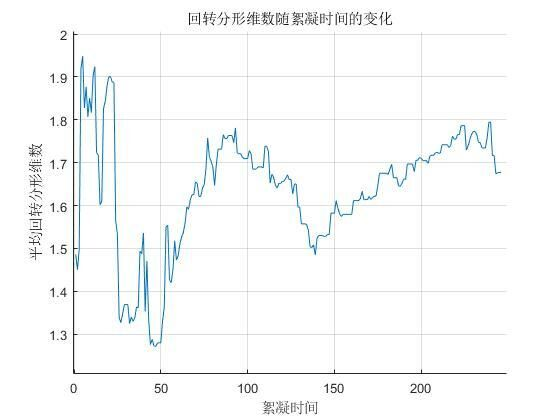
\includegraphics[width=0.6\textwidth]{results/time.png}
    \caption{分形维数随絮凝时间变化关系图}
\end{figure}

从图像可见,平均分形维数在模拟中不断波动,但逐渐趋于一个稳定的值,说明所取的终止条件较为合理。这也说明了第二种回转半径法算得的分形维数是一个合理的、可收敛的特征值。

\subsection{DLA下,初始粒子体积密度与最终$d_f$的关系}
取$L= 100, l = 2$,在[1000, 10000]区间间隔1000取$n$,采集$d_f$数据点,得到图2。
\begin{figure}[htbp]
    \centering
    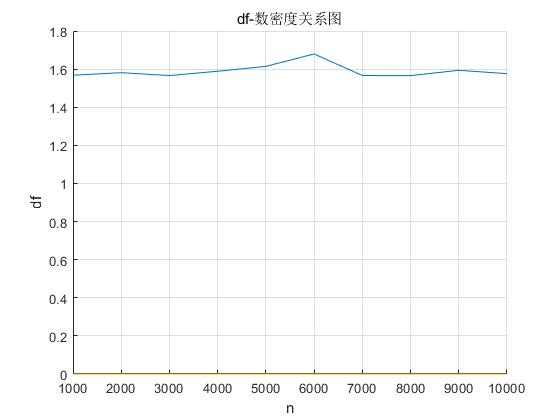
\includegraphics[width=0.6\textwidth]{results/n.png}
    \caption{$d_f$与粒子数关系图}
\end{figure}

在同样的体积内,取不同的粒子数即可得到不同的初始粒子体积密度。从图中来看,分形维数与粒子数没有呈现可见的相关性,说明在给定范围内与初始粒子体积密度无关。

\subsection{DLA下,粒子布朗运动步长与最终$d_f$的关系}
取$L = 100, n = 5000$,在[1, 3]区间间隔0.2取$l$,采集$d_f$数据点,得到图3。
\begin{figure}[htbp]
    \centering
    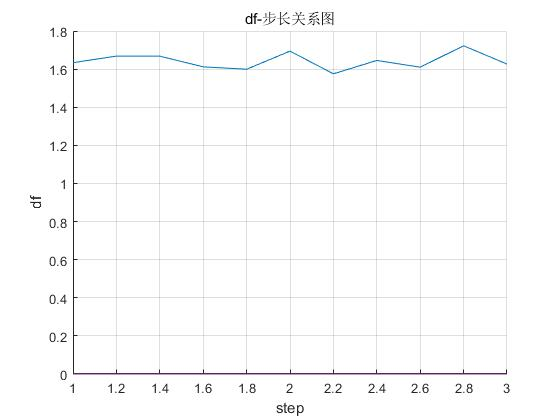
\includegraphics[width=0.6\textwidth]{results/step.png}
    \caption{$d_f$与粒子布朗运动步长关系图}
\end{figure}

从图中来看,分形维数与粒子布朗运动步长没有呈现相关性。在其他条件相同的情况下,布朗运动步长与温度成正相关,因此说明在给定的步长范围内,外界温度对絮凝体的分形维数没有可见的影响。

\subsection{RLA粘连概率对最终$d_f$的影响}
取$L = 100, n = 5000, l = 2$,在[0.2, 1]区间间隔0.1取粘连概率$p$,采集$d_f$数据点,得到图4。
\begin{figure}[htbp]
    \centering
    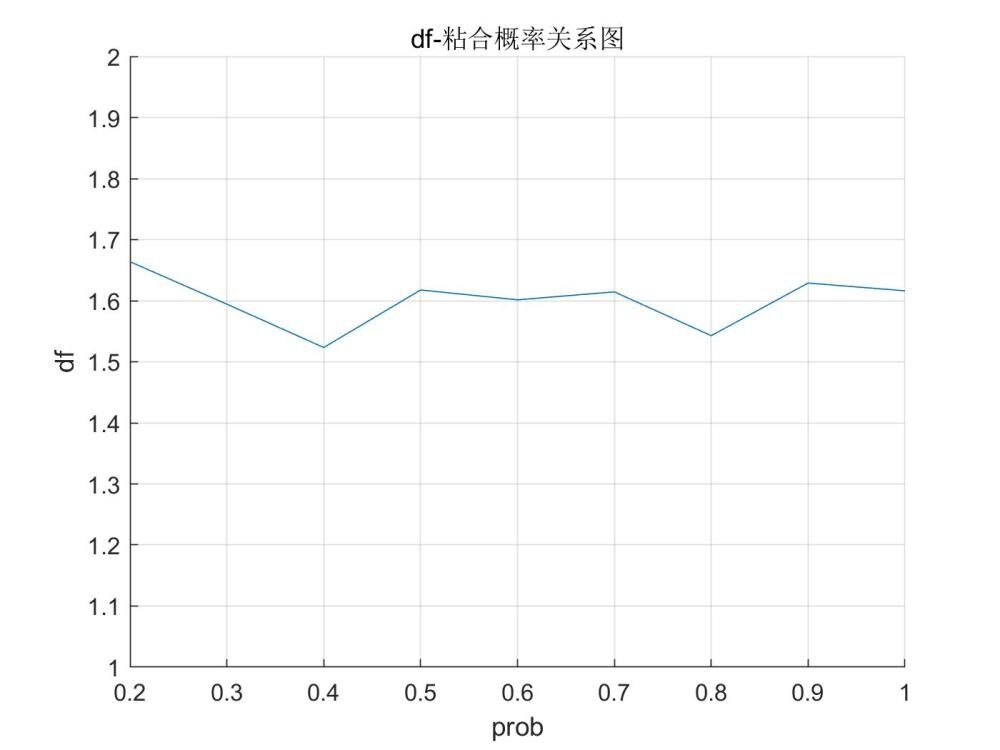
\includegraphics[width=0.6\textwidth]{results/prob.png}
    \caption{$d_f$与RLA粘连概率关系图}
\end{figure}

从图中来看,分形维数在1.55到1.65间波动,与RLA粘连概率也没有呈现出明显的相关性。

\section{结论和反思}
上述的四个模拟实验结果有些超出我们的预料,因为在一定时间以后,絮凝体的分形维数似乎是一个确定的、不变的值,大约为1.6,不随粒子体积密度、粒子布朗运动步长或粘连概率变化而改变。一个考虑到的原因是本实验中终止条件不是传统的“一定时间之后”,而是“团簇数目小于等于粒子数的0.4倍”。这或许意味着,在达到相同团簇数目占比(即凝聚占比)的条件下,絮凝体的分形维数就是一个固定的值。

由于时间原因,我们没能更加深入地研究得到有哪些影响DLA/RLA模型分形维数的因素,但通过本实验我们似乎说明了絮凝体的分形维数是一个值得注意的固定特征值。这也让我们对分形数学和凝聚等自然规律之间的联系有了新的认识。


\end{document}
